\documentclass[12pt,a4paper]{article}\usepackage[]{graphicx}\usepackage[]{color}
%% maxwidth is the original width if it is less than linewidth
%% otherwise use linewidth (to make sure the graphics do not exceed the margin)
\makeatletter
\def\maxwidth{ %
  \ifdim\Gin@nat@width>\linewidth
    \linewidth
  \else
    \Gin@nat@width
  \fi
}
\makeatother

\definecolor{fgcolor}{rgb}{0.345, 0.345, 0.345}
\newcommand{\hlnum}[1]{\textcolor[rgb]{0.686,0.059,0.569}{#1}}%
\newcommand{\hlstr}[1]{\textcolor[rgb]{0.192,0.494,0.8}{#1}}%
\newcommand{\hlcom}[1]{\textcolor[rgb]{0.678,0.584,0.686}{\textit{#1}}}%
\newcommand{\hlopt}[1]{\textcolor[rgb]{0,0,0}{#1}}%
\newcommand{\hlstd}[1]{\textcolor[rgb]{0.345,0.345,0.345}{#1}}%
\newcommand{\hlkwa}[1]{\textcolor[rgb]{0.161,0.373,0.58}{\textbf{#1}}}%
\newcommand{\hlkwb}[1]{\textcolor[rgb]{0.69,0.353,0.396}{#1}}%
\newcommand{\hlkwc}[1]{\textcolor[rgb]{0.333,0.667,0.333}{#1}}%
\newcommand{\hlkwd}[1]{\textcolor[rgb]{0.737,0.353,0.396}{\textbf{#1}}}%

\usepackage{framed}
\makeatletter
\newenvironment{kframe}{%
 \def\at@end@of@kframe{}%
 \ifinner\ifhmode%
  \def\at@end@of@kframe{\end{minipage}}%
  \begin{minipage}{\columnwidth}%
 \fi\fi%
 \def\FrameCommand##1{\hskip\@totalleftmargin \hskip-\fboxsep
 \colorbox{shadecolor}{##1}\hskip-\fboxsep
     % There is no \\@totalrightmargin, so:
     \hskip-\linewidth \hskip-\@totalleftmargin \hskip\columnwidth}%
 \MakeFramed {\advance\hsize-\width
   \@totalleftmargin\z@ \linewidth\hsize
   \@setminipage}}%
 {\par\unskip\endMakeFramed%
 \at@end@of@kframe}
\makeatother

\definecolor{shadecolor}{rgb}{.97, .97, .97}
\definecolor{messagecolor}{rgb}{0, 0, 0}
\definecolor{warningcolor}{rgb}{1, 0, 1}
\definecolor{errorcolor}{rgb}{1, 0, 0}
\newenvironment{knitrout}{}{} % an empty environment to be redefined in TeX

\usepackage{alltt}
%%%%%%%%%%%%%%%%%%%%%%%%%%%%%%%%%%%%%%%%%%%%%%%%%%%%%%%%%%%%%%%%%%%%%%%%%%%%%%%%%%%
% knitr stuff for R code chunks
% always need this code chunk, never mess with it!

%%%%%%%%%%%%%%%%%%%%%%%%%%%%%%%%%%%%%%%%%%%%%%%%%%%%%%%%%%%%%%%%%%%%%%%%%%%%%%%%%%%

%%%%%%%%%%%%%%%%%%%%%%%%%%%%%%%%%%%%%%%%%%%%%%%%%%%%%%%%%%%%%%%%%%%%%%%%%%%%%%%%%%%
\usepackage{helvet} 
\renewcommand{\familydefault}{\sfdefault}
\usepackage{a4wide}
\usepackage{ucs}
\usepackage[utf8x]{inputenc}
\usepackage[english]{babel} % Language packages
\usepackage{graphicx}
\usepackage{cite}
\usepackage[absolute]{textpos}
\usepackage{tabularx} 
\usepackage{tabulary} 
\usepackage{fancyhdr}
\usepackage[table]{xcolor}
\usepackage{longtable} % for long tables
\pagestyle{fancy}
\headsep=50pt
\listfiles % list the package versions in the log file
%%%%%%%%%%%%%%%%%%%%%%%%%%%%%%%%%%%%%%%%%%%%%%%%%%%%%%%%%%%%%%%%%%%%%%%%%%%%%%%%%%%
% header information table, using fancyhdr
\lhead{}
\fancyhead[C]{{\footnotesize
\textblockorigin{-18pt}{-2pt}
\begin{textblock*}{10cm}(2cm,1cm)

\includegraphics[height=1.5cm,keepaspectratio]{figures/logo/NYULMC_white.jpg}
\end{textblock*}
\begin{tabularx}{1.0\textwidth}{|l|X|l|l|}
\hline 
\textbf{556 PANEL} & \textbf{CLINICAL REPORT} & \textbf{Date:}  &  \today \\ 
% \hline
\multicolumn{2}{|l|}{PATIENT NAME GOES HERE} & \textbf{PATIENT ID} &  999999 \\ 
% \hline
\multicolumn{2}{|l|}{Diagnosis: {\scriptsize Squamous epithelial kiwi carcinoma}} & \textbf{Misc. ID:} & 999999  \\ 
% \hline
\end{tabularx}}}
\rhead{}
%%%%%%%%%%%%%%%%%%%%%%%%%%%%%%%%%%%%%%%%%%%%%%%%%%%%%%%%%%%%%%%%%%%%%%%%%%%%%%%%%%%
\IfFileExists{upquote.sty}{\usepackage{upquote}}{}
\begin{document}
\section*{Case Images}
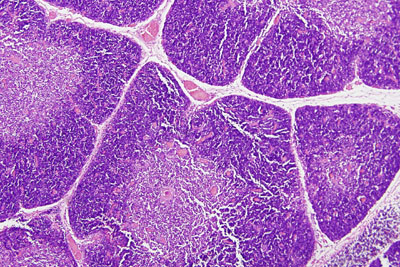
\includegraphics[height=4cm,keepaspectratio]{figures/histology/athymus2.jpg}
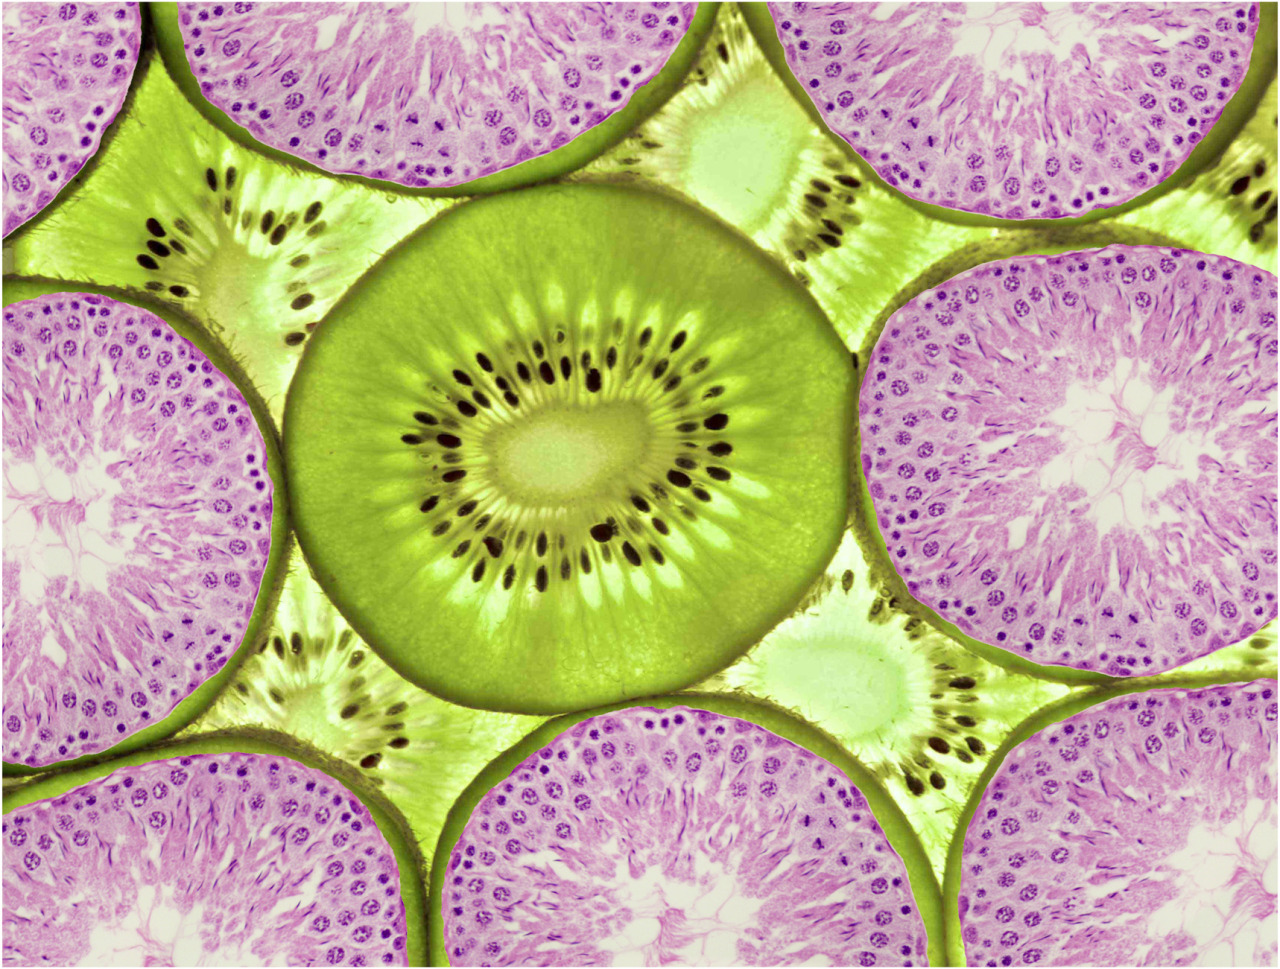
\includegraphics[height=4cm,keepaspectratio]{figures/histology/bhistolokiwi.jpg}
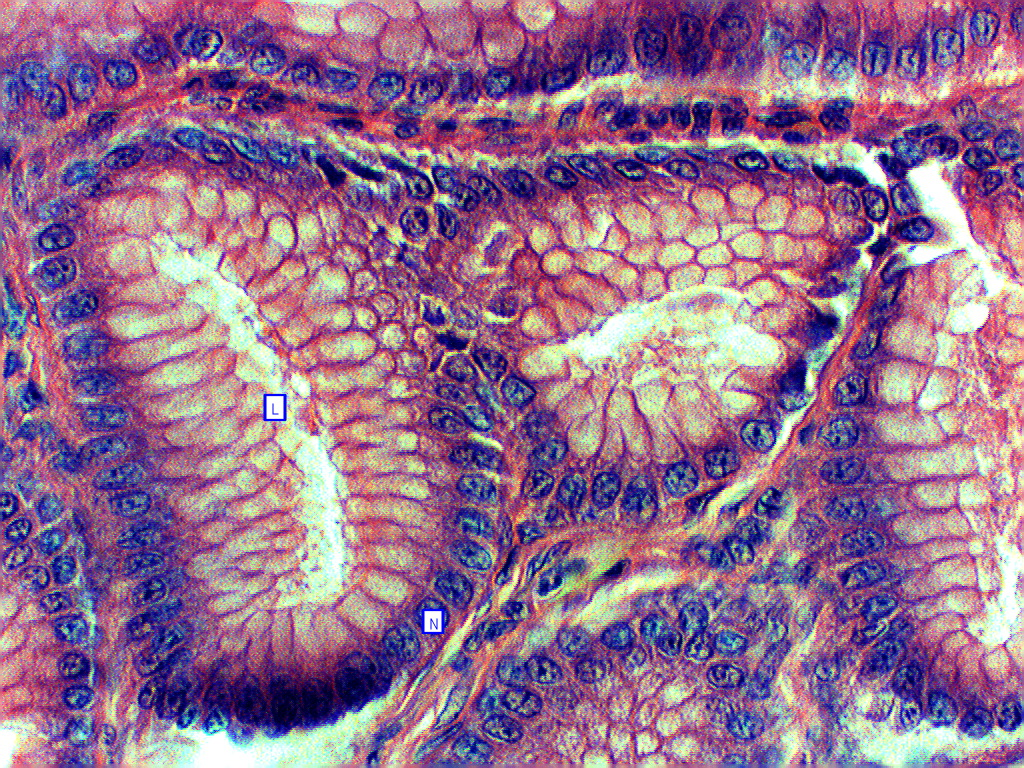
\includegraphics[height=4cm,keepaspectratio]{figures/histology/SimpleColumnarEpithelium1_0.jpg}

%%%%%%%%%%%%%%%%%%%%%%%%%%%%%%%%%%%%%%%%%%%%%%%%%%%%%%%%%%%%%%%%%%%%%%%%%%%%%%%%%%%
\section*{Results}
\textbf{GENOMIC ALTERATIONS:} Summary \\
 \\
Somatic alterations in clinically relevant genes. \\
 \\
A set of  556 genes were investigated.  42  variants were found among these.\\
 \\
\textbf{Clinically Relevant Genomic Alterations} \\
 \\
% latex table generated in R 3.2.3 by xtable 1.8-2 package
% Mon Mar  7 21:03:21 2016
\begingroup\footnotesize
\begin{longtable}{ll}
  \hline
Gene.refGene & AAmatch \\ 
  \hline
JAK1 & G307S \\ 
  ARID1A & T1743M \\ 
  RET & R897Q \\ 
  PTEN & R233 \\ 
  FANCF & A186V \\ 
  ATM & H1352R \\ 
  KMT2A & E2416K \\ 
  ATM & R2719H \\ 
  ERBB3 & E925K \\ 
  KRAS & G13D \\ 
  KMT2D & R5007W \\ 
  KRAS & G12V \\ 
  IRS2 & P548T \\ 
  FLT1 & V1331I \\ 
  BLM & V4A \\ 
  IGF1R & S72N \\ 
  TSC2 & A1257V \\ 
  CTCF & Q44R \\ 
  TP53 & T284P \\ 
  TP53 & R306 \\ 
  BCL2 & V15M \\ 
  IDH1 & R132H \\ 
  IDH1 & R132C \\ 
  ZNF217 & M410V \\ 
  GNAS & R844H \\ 
  CRKL & R164Q \\ 
  SOX10 & R215Q \\ 
  EPHB1 & V562I \\ 
  FBXW7 & R465H \\ 
  EPHA5 & S873Y \\ 
  RICTOR & M1341V \\ 
  MAP3K1 & S939C \\ 
  APC & P2346S \\ 
  FLT4 & E58K \\ 
  FANCE & P445S \\ 
  EGFR & V769M \\ 
  BRAF & V600E \\ 
  PIK3CG & D358Y \\ 
  KMT2C & T3017K \\ 
  PTCH1 & E52G \\ 
  SYK & G5S \\ 
  BCOR & S26R \\ 
   \hline
\hline
\end{longtable}
\endgroup

%%%%%%%%%%%%%%%%%%%%%%%%%%%%%%%%%%%%%%%%%%%%%%%%%%%%%%%%%%%%%%%%%%%%%%%%%%%%%%%%%%%
\clearpage
\section{System and Session Information}\label{session}
\LaTeX{} version: \LaTeXe~ \fmtversion
\begin{knitrout}\footnotesize
\definecolor{shadecolor}{rgb}{0.969, 0.969, 0.969}\color{fgcolor}\begin{kframe}
\begin{alltt}
\hlkwd{system}\hlstd{(}\hlstr{'uname -srv'}\hlstd{,}\hlkwc{intern}\hlstd{=T)}
\end{alltt}
\begin{verbatim}
## [1] "Linux 2.6.32-573.18.1.el6.x86_64 #1 SMP Tue Feb 9 22:46:17 UTC 2016"
\end{verbatim}
\begin{alltt}
\hlkwd{sessionInfo}\hlstd{()}
\end{alltt}
\begin{verbatim}
## R version 3.2.3 (2015-12-10)
## Platform: x86_64-redhat-linux-gnu (64-bit)
## Running under: CentOS release 6.7 (Final)
## 
## locale:
##  [1] LC_CTYPE=en_US.UTF-8       LC_NUMERIC=C              
##  [3] LC_TIME=en_US.UTF-8        LC_COLLATE=en_US.UTF-8    
##  [5] LC_MONETARY=en_US.UTF-8    LC_MESSAGES=en_US.UTF-8   
##  [7] LC_PAPER=en_US.UTF-8       LC_NAME=C                 
##  [9] LC_ADDRESS=C               LC_TELEPHONE=C            
## [11] LC_MEASUREMENT=en_US.UTF-8 LC_IDENTIFICATION=C       
## 
## attached base packages:
## [1] stats     graphics  grDevices utils     datasets  methods   base     
## 
## other attached packages:
## [1] Hmisc_3.17-1    ggplot2_2.0.0   Formula_1.2-1   survival_2.38-3
## [5] lattice_0.20-33 xtable_1.8-2    knitr_1.12.3   
## 
## loaded via a namespace (and not attached):
##  [1] Rcpp_0.12.3         cluster_2.0.3       magrittr_1.5       
##  [4] splines_3.2.3       munsell_0.4.2       colorspace_1.2-6   
##  [7] stringr_1.0.0       highr_0.5.1         plyr_1.8.3         
## [10] tools_3.2.3         nnet_7.3-12         grid_3.2.3         
## [13] gtable_0.1.2        latticeExtra_0.6-26 gridExtra_2.0.0    
## [16] RColorBrewer_1.1-2  formatR_1.2.1       acepack_1.3-3.3    
## [19] rpart_4.1-10        evaluate_0.8        stringi_1.0-1      
## [22] scales_0.3.0        foreign_0.8-66
\end{verbatim}
\end{kframe}
\end{knitrout}
\end{document}
